\documentclass[a4paper,oneside,14pt, extrafontsizes]{memoir}

 \usepackage{graphicx}
\usepackage{verbatim}
\renewcommand{\familydefault}{\sfdefault}
\chapterstyle{demo2}

\title{\emph{Conceptual Modeling Language}\\Specification\\ \small{Version 1.0 (Draft)}}
\author{Quenio Cesar Machado dos Santos\\
\small{Universidade Federal de Santa Catarina}\thanks{
Initially developed as part of the author's Bachelor Technical Report in Computer Sciences}}
\date{July 2017}

\makeatletter
\newcommand{\verbatimfont}[1]{\renewcommand{\verbatim@font}{\ttfamily#1}}
\makeatother

\begin{document}

\begin{titlingpage}
\maketitle
\end{titlingpage}

\frontmatter

\begin{KeepFromToc}

\clearpage
\tableofcontents

\clearpage
\listoffigures

\clearpage
\listoftables

\end{KeepFromToc}

\mainmatter

\chapter{Introduction}
This document specifies the \emph{Conceptual Modeling Language}, or CML for short.
CML enables the modeling of the information of software systems.
It focuses on modeling the structural aspects of such systems,
having less emphasis on the behavioral aspects.
Using CML,
it is possible to represent the information as understood by the system users,
while disregarding its physical organization as implemented by target languages or technologies.

The CML compiler has:
\begin{itemize}
\item as \emph{input},
source files defined using its own conceptual language (as specified in this document),
which provides an abstract syntax similar to (but less comprehensive than) a combination of UML \cite{uml} and OCL \cite{ocl};
\item and, as \emph{output},
any target languages based on extensible templates,
which may be provided by the compiler's base libraries, by third-party libraries, or even by developers.
\end{itemize}

Section \ref{sec:compiler} will provide an overview of the CML compiler's architecture.
Section \ref{sec:org} describes the organization and notation
used in the remainder of this document.


\chapter{Compiler}
\label{ch:compiler}
The CML compiler's overall architecture follows the standard compiler design literature \cite{torben}. An overview diagram of the architecture is shown in figure \ref{fig:overview}.

\begin{figure}
\centering
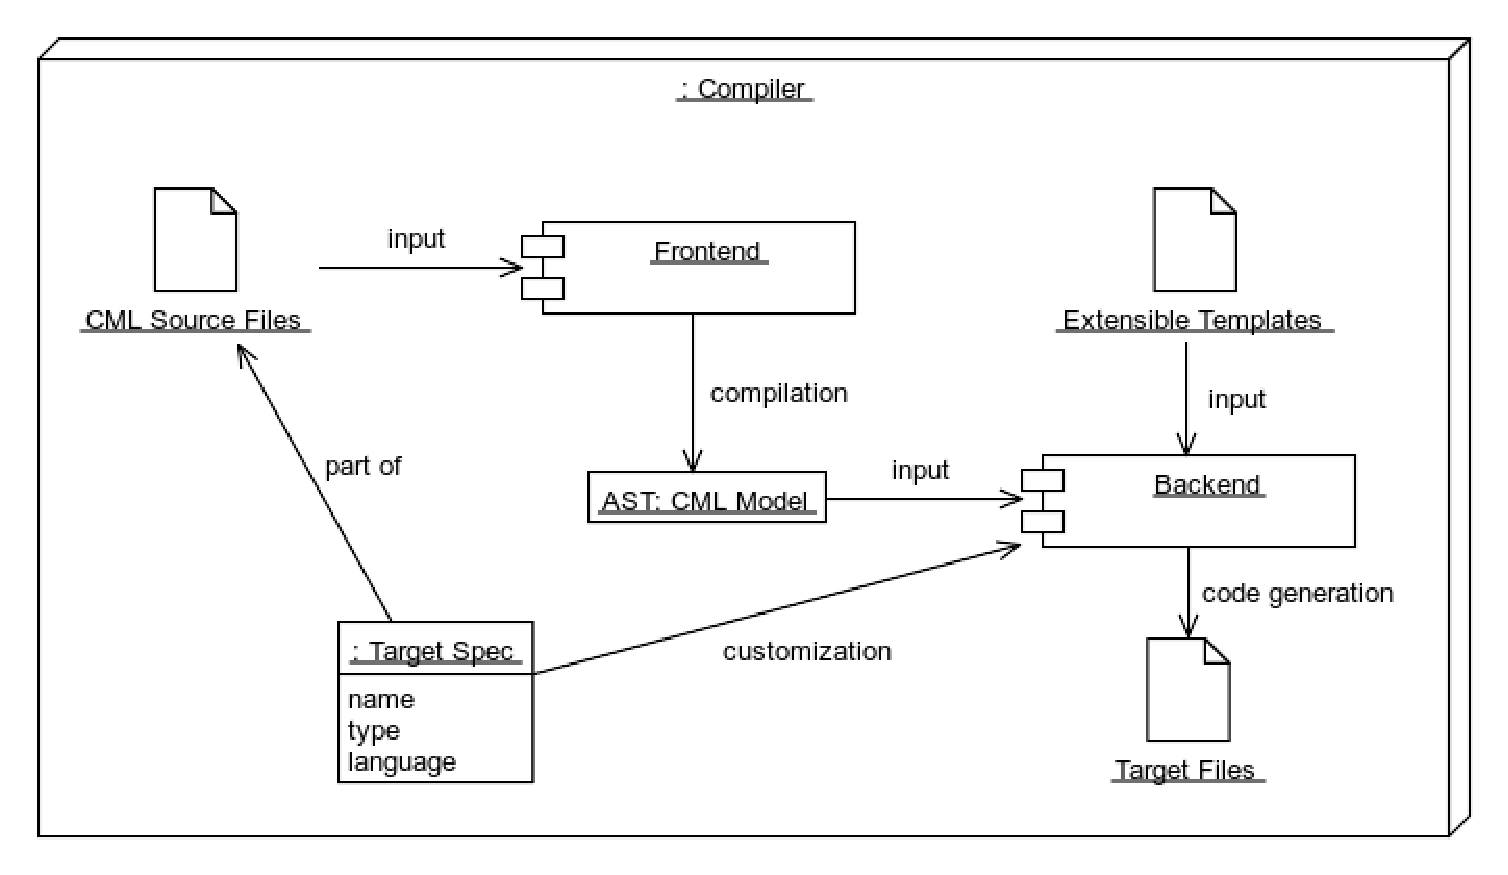
\includegraphics[width=\textwidth]{compiler/figure-overview}
\caption{An architectural overview of the CML compiler.}
\label{fig:overview}
\end{figure}

The two main components of the compiler,
and the artifacts they work with,
are presented in the next subsections.


\chapter{Concepts}

\begin{figure}
\verbatimfont{\small}
\begin{framed}
\verbatiminput{grammar/Concepts.txt}
\end{framed}
\caption{Concept Declaration Syntax}
\label{fig:concept-syntax}
\end{figure}

\section{Properties}\label{sec:properties}

\begin{figure}
\verbatimfont{\small}
\begin{framed}
\verbatiminput{grammar/Properties.txt}
\end{framed}
\caption{Properties Declaration Syntax}
\label{fig:properties-syntax}
\end{figure}

\section{Inheritance}\label{sec:inheritance}


\chapter{Associations}

\section{Unidirectional Associations}\label{sec:assoc-unidir}

\section{Bidirectional Associations}\label{sec:assoc-bidir}

\section{Collection Types}\label{sec:collection-types}


\chapter{Values}
\input{values/values.tex}

\chapter{Expressions}

\chapter{Targets}
\label{ch:targets}

\chapter{Modules and Libraries}

\appendix

\chapter{Concrete Syntax (Grammar)}
\clearpage
\section{ANTLR Grammar}

\begin{framed}
\verbatimfont{\small}
\begin{verbatim}
// Compilation Units:
\end{verbatim}
\verbatiminput{grammar/CompilationUnits.txt}
\begin{verbatim}
// Concept Declarations:
\end{verbatim}
\verbatiminput{grammar/Concepts.txt}
\begin{verbatim}
// Property Declarations:
\end{verbatim}
\verbatiminput{grammar/Properties.txt}
\begin{verbatim}
// Type Declarations:
\end{verbatim}
\verbatiminput{grammar/Types.txt}
\begin{verbatim}
// Target Declarations:
\end{verbatim}
\verbatiminput{grammar/Targets.txt}
\begin{verbatim}
// Names:
\end{verbatim}
\verbatiminput{grammar/Names.txt}
\begin{verbatim}
// Literals:
\end{verbatim}
\verbatiminput{grammar/Literals.txt}
\verbatiminput{grammar/Ignored.txt}
\end{framed}


\chapter{Abstract Syntax (Metamodel)}
\input{metamodel.tex}

\chapter{Abstract Syntax Tree (Instantiation)}
\input{ast.tex}

\backmatter

\bibliographystyle{plain}
\bibliography{references}

\end{document}
